\documentclass[a4paper,12pt]{report}

\usepackage{rapportutc}
\usepackage{gensymb}
\usepackage{float}

\floatplacement{figure}{h} % Indique de placer les figures là où elles sont déclarées

\title{Amélioration et conception de workflows}
\author{Erwan Normand}
\date{\today}

\uv{Rapport de stage TN09}
\semestre{Automne 14}
\branche{Université de Technologie}
\filiere{de Compiègne}
\specialite{Génie Informatique}

\suiveurutc{Mohamed Sallak}
\suiveurets{Nicolas Burtey}
\entreprise{VideoStitch}
\logoets{
\includegraphics[width=6cm]{images/videostitch.jpg}}
\lieustage{Paris}


\begin{document}

\pagedetitre

\chapter*{Remerciements}
Je tiens à remercier tout d'abord l'UTC et VideoStitch pour m'avoir permis de réaliser ce stage technique d'assistant ingénieur. Ces 7 mois très riches m'ont permis de constituer une première expérience technique et professionnelle solide en ingénierie logicielle et de réaliser la transition de première année commune du Génie Informatique de l'UTC à la filière de spécialisation d'Ingénierie des Connaisances et des Systèmes d'Informations.
\\
\newline
Je remercie sincèrement Nicolas Burtey, pour m'avoir accueilli dans son entreprise et pour la confiance qu'il m'a témoignée en acceptant ma candidature.\\
Et je remercie toute l'équipe, ingénieurs, commerciaux, et stagiaires de VideoStitch avec qui j'ai pu longuement travailler : Andrés Peralta, Nicolas Lopez, Julien Fond, Henri Rebecq, Nils Duval, Rodolphe Fouquet, Wieland Morgenstern, Raphaël Lemoine, Jean Vittor, Aksel Piran, Liesbeth De Mey, Florent Melchior, Rodolphe Chartier, Alexis Pontin ainsi que les deux UTCéens avec qui j'ai effectué mon stage : Marie Chatelin et Jean Duthon. Merci pour leurs aides, les nombreux partages et connaissances échangés. Venir travailler fut un plaisir et une motivation tous les jours grâce à eux tous et à l'excellente ambiance dans l'équipe.
\\
\newline
Je remercie l'incubateur Télécom Paris Tech de Paris XIV où s'est déroulé le stage.
\\
\newline
Enfin, je remercie toutes les personnes qui m'ont consacré de leur temps au support de leurs produits, et merci à ceux qui les ont conçus. Notre travail est entouré d'outils qui innovent sans cesse et où nous prenons notre place. Il est bon de se rappeller que toute innovation a ses fondations; et j'espère que les briques que j'ai apportées seront la source de nouvelles idées.


\tableofcontents
\addcontentsline{toc}{chapter}{Sommaire}

\chapter*{Introduction}
\addcontentsline{toc}{chapter}{Introduction}
Dans le cadre de la formation ingénieur de l'Université de Technologie de Compiègne,
le 3\up{e} semestre (bac+4) est consacré à un stage de 24 semaines d'assistant ingénieur.
Cette période de travail se déroule dans le milieu professionel, du secteur
privé ou public, dans une optique d'une première expérience longue, qui a pour
objectif une confrontation au monde du travail, de comprendre ses contraintes et 
enjeux, et enfin de tirer un enseignement d'une mise en application pratique des
connaissances reçues à l'UTC jusqu'ici.\\
\newline
Mon stage s'est déroulé à VideoStitch, éditeur de logiciels de vidéo panoramique
à 360\degree, dans les locaux de Telecom Paris Tech dans le 14\up{ème} arrondissement de Paris. 
Il a été précédé d'un CDD de 7 semaines, totalisant avec le stage d'une période 
de travail s'étendant du 15 juillet 2014 au 13 février 2015.\\
\newline
Ce rapport est consacré au compte rendu de ce travail; plus particulièrement aux
missions qui m'ont été confiées, des difficultés rencontrées et des solutions
proposées ainsi que leurs apprentissages et bilans.


\chapter{Présentation de l'entreprise}
ping
\section{VideoStitch}
\subsection{Présentation générale}
\begin{wrapfigure}{r}{35mm}
    
\includegraphics{images/videostitch.png}
    \caption{Logo de VideoStitch}
\end{wrapfigure}
VideoStitch est une entreprise française d'édition de logiciels, qui conçoit et vend des logiciels de capture, de montage, de montage, de diffusion et de lecture de vidéos panoramiques à 360\degree. Elle s'intéresse par extension au marché de la réalité virtuelle, ou encore appellée VR.
Son site internet est à l'adresse suivante : \url{http://www.video-stitch.com/}.\\
C'est une Société à Actions Simplifiées (SAS) basée sur Paris, qui emploie moins d'un dizaine de personnes actuellement. 
La plupart ayant été embauchés il y a quelques mois, c'est une société en forte croissance salariale. 
Nicolas Burtey en est le président.

\subsection{Historique}
VideoStitch a été fondée par ce même Nicolas Burtey en janvier 2012.\\
Photographe diplômé de l'Ecole Lumière, s'étant fait connaître par la photo panoramique et la photo fish-eye, M. Burtey évolue par la suite dans le domaine de la vidéo panoramique.\\
\begin{wrapfigure}{l}{50mm}
    
\includegraphics[width=50mm]{images/loopin.png}
    \caption{Logo de Loop'in}
\end{wrapfigure}
Il crée sa société de production vidéo, Loop'In, avec laquelle il réalise une certain nombre de vidéos panoramiques à 360\degree pour de nombreux clients. Un certain nombre d'exemples de ces vidéos sont disponibles à cette adresse : \url{http://www.loop-in.com/galerie/}.
La vidéo panoramique, inconnue du grand public et étant un procédé très jeune, est lente et difficile à réaliser, beaucoup de tâches devant être faites de manière manuelle et répétitive, avec des outils inadaptés car non prévus à cette utilisation.
Si la création de photos panoramiques et à 360\degree est aisée, il manque toutefois un logiciel complet et mature permettant l'édition et le montage de vidéos panoramiques.\\
\newline
M. Burtey décide alors de créer VideoStitch et de concevoir cet outil. C'est une petite équipe de trois personnes qui se forme ainsi pour concevoir leur premier logiciel d'éditions et de montage de vidéos panoramiques : VideoStitch Studio.\\
Quand ce logiciel atteint une version stable, en 2014, VideoStitch oriente alors ses efforts vers un nouveau logiciel, Vahana VR, permettant cette fois-ci une réalisation et une diffusion en direct de vidéos panoramiques à 360\degree.\\
\newline
Le but de la société est de permettre une réalisation aisée et de qualité de vidéos panoramiques à 360\degree, de la capture des images à la diffusion de la vidéo finale, en passant par sa réalisation complète.


\section{Les marchés et les produits}
% La vidéo 360 panoramique et la VR, les principaux acteurs, bref historique et portrait actuel

\section{Produits et stratégies de l'entreprise}
% Studio, Vahana VR
% Player, réseaux sociaux, salons, rencontres entreprises

\section{Organisation de l'entreprise}
% Organisation de l'entreprise : les différentes personnes et articulation des rôles et des tâches.
% Organisation du travail : Agile/Scrum, JIRA, Confluence, Github et autres outils.

\section{Stratégies pour l'avenir et ambitions}
% Analyse de l'avenir des marchés, stratégies de positionnement et d'investissement, ambitions

\chapter{Présentation du stage}

\section{Le sujet}
Le titre du sujet du stage était initialement \enquote{\textit{Developer C++/Qt.
work on a challenging and immersive 360 video software}}.\\
Bien que très général, le domaine de l'entreprise se trouvait être très intéressant
et durant l'entretien qui s'est déroulé à la mi-mai, quelques sujets ont été
développés~: M. Burtey m'a donc proposé de travailler sur le Player d'une part,
à la suite d'Alexis Pontin et pour terminer son travail, et d'une autre part de
travailler au développement du nouveau produit VideoStitch Live, renommé par la
suite en Vahana VR, qui allait débuter dans quelques semaines.\\
M. Burtey n'était pas encore certain du lancement du développement de Vahana VR, 
et envisageait également à la conception du \textit{stitch} stéréoscopique 3D\footnote{Qui
consiste, brièvemenent, en la conception de deux équirectangulaires pour la même
scène filmée~: un pour chaque oeil en exploitant l'effet de la parallaxe, recréant 
un effet de relief\cite{videostitch-stereo}
\cite{image-stereoscopique}}, il me proposa également de travailler au développement
de la prise en charge de la 360 stéréo dans Videostitch Studio. Le sujet final serait
décidé la première semaine du stage.\\
\newline
Le stage fut finalement précédé par un CDD à temps partiel de 7 semaines, mes missions
se sont alors simplement étendues du début du CDD à la fin du stage, c'est-à-dire 
7 mois.\\
Le sujet réel a donc été arrêté à deux missions\footnote{La 3D s'est révélée être 
une tâche trop ardue, après un rapide état de l'art du sujet par les ingénieurs~: 
même si les articles de recherche et brevets sont nombreux, aucune application 
industrielle n'a encore aujourd'hui aboutis.}~:
\begin{enumerate}
  \item L'intégration de VideoStitch Player et de Vahana VR au flux de développement
  logiciel et d'intégration continue de VideoStitch, tout en assurant une maintenance sur le Player.
  \item La conception, le développement et le déploiement d'un système
  d'intégration de caméras et de cartes d'acquisitions dans Vahana VR.
\end{enumerate}
Ces deux missions trouvent comme sujet commun \emph{l'amélioration de \textit{workflow}
dans et pour les usages des ingénieurs de VideoStitch}. La première consiste en 
ce sens à l'amélioration du système et des outils de développement et d'intégration des logiciels
de l'entreprise; et la seconde permet par un système indépendant et modulaire de
nouvelles capacités à Vahana VR.

\section{Les méthodes de travail}

\section{Les outils utilisés}


\chapter{Amélioration du flux de développement}
\epigraph{Il semble que la perfection soit atteinte, non quand il n'y a plus 
rien à ajouter mais quand il n'y a plus rien à retrancher}{--- \small{\textup{Saint-Exupéry,
Terre des hommes}}}

\section{Définition de la mission}
\subsection{Contexte}
Au début de ce stage, mi-juillet, la première tâche fut la prise de contact avec 
les méthodes de travail, les outils utilisés, les logiciels développés, et leurs
\textit{workflows} de développement. En effet, si jusqu'ici seul Studio était développé, Alexis
Pontin venait de terminer le projet du Player, et le développement de Vahana
VR commençait. Studio utilisait alors une architecture de développement particulière
et le Player tout comme Vahana VR commençaient leur développement selon leurs propres
\textit{workflows}.\\
\newline
Ce qui est appelé \textit{workflow} dans ce rapport est un terme pour désigner le 
\enquote{flux de travaux, [c'est-à-dire] une suite de tâches et
d'opérations effectuées par [...] un groupe de personnes}\cite{workflow}, ici l'équipe de développement
de VideoStitch~: c'est une représentation des différentes tâches à accomplir pour, depuis un poste de travail vierge, 
l'installer et pouvoir travailler un des produits de l'entreprise, le compiler et le distribuer.
Ce n'est pas l'architecture des logiciels en eux même, ni leur développement,
mais comment, à partir des sources et des dépendances, il possible d'arriver au produit
compilé et distribuable au client.\\
Ce processus met en \oe uvre plusieurs concepts qui s'articulent autour du développement
logiciel proprement dit~:\cite{software-build}\cite{build-automation}
\begin{itemize}
  \item La gestion de versions, assurée ici avec Git\cite{gestion-versions}, qui permet
  de récupérer les codes sources.
  \item La chaîne de compilation, dépendante de l'OS cible et automatisée avec Buildbot 
  \cite{chaine-compilation}\cite{integration-continue}.
  \item Les tests d'intégration\cite{integration-continue} réalisés par Buildbot.
  \item La création des installateurs et leur mise à disposition sur une page de téléchargement interne.
\end{itemize}
\ \newline
Cette mission porte essentiellement sur l'amélioration de la chaîne de compilation
pour les applications de VideoStitch, VideoStitch Studio, Vahana VR et VideoStitch
Player, et la création des installateurs. Ce travail a été très complémentaire avec
celui de Jean Duthon, qui a amélioré le \textit{workflow} de développement de VideoStitch SDK,
la gestion des versions et les tests d'intégration.

\subsection{Le \textit{workflow} de développement de VideoStitch Studio} 
Les codes sources et les dépendances avaient été réparties en quatre dépôts Git~: 
\begin{itemize}
  \item VideoStitch-lib, contenant le VideoStitch SDK
  \item VideoStitch-base, contenant des code sources partagés avec le dépôt du VideoStitch Player
  \item VideoStitch-apps, contenant VideoStitch Studio
  \item VideoStitch-deps, contenant les dépendances Windows de VideoStitch Studio 
  nécessaires à sa compilation\footnote{Présentées plus en détails dans \cf{integration-dependances-player}}
\end{itemize}
Sous les systèmes Linux et OS X, il a été décidé d'utiliser les gestionnaires
de paquets apt et Macport pour installer les dépendances logicielles de Studio. Pour
Windows, le dépôt VideoStitch-deps tenait les dépendances sous des versions stables et testées.\\
\newline
Compiler et créer l'installateur de Studio depuis un poste de travail vierge requérait alors
certaines étapes, représentées sous forme d'un diagramme de séquence sur la figure~\ref{workflow-studio}.
Ces étapes étaient essentiellement des appels à des commandes et à des scripts internes
(écrits en bash pour Linux / Mac et en batch pour Windows) pour faire le lien entre les trois dépôts~:
\begin{itemize}
  \item Cloner les dépôts VideoStitch-deps, VideoStitch-base et VideoStitch-apps
  \item Générer une version du logiciel via un script présent sur VideoStitch-apps
  \item Récupérer la dernière version du VideoStitch SDK compilée par Buildbot, 
  via un script présent sur VideoStitch-apps
  \item Copier, via un script présent sur VideoStitch-base, les codes sources partagés
  \item Copier, via un script batch présent sur VideoStitch-deps, les dépendances pour Windows
  \item Générer le Makefile avec le logiciel qmake fournis avec Qt
  \item Compiler avec le logiciel jom fournis avec Qt
  \item Générer l'installateur avec un script présent sur VideoStitch-apps
\end{itemize}
\begin{figure}
  \centering
  \caption{Diagramme de séquence du \textit{workflow} de Studio (07/2014)}
	\label{workflow-studio}
\end{figure}

\subsection{Problématique}
Représenter ce flux présente l'intérêt de pouvoir ensuite le simplifier et d'automatiser
un maximum des processus requis. Et cela était devenu nécessaire, pour deux raisons~:
\begin{itemize}
  \item L'entreprise commençait sa croissance, impliquant de former les nouveaux arrivants
  à un \textit{workflow} de développement devenue complexe à mesure du temps. Il fallait en
  simplifier le fonctionnement maintenant que Studio et son développement était
  devenus matures\footnote{La première version était sortie, et la bêta de la seconde
  version était en cours}, ce qui permettrait de gagner en efficacité sur le développement
  proprement dit.
  \item Vahana VR et le Player avaient débuté leurs développements; pourtant ces trois
  produits, avec Studio, ont en commun l'utilisation de VideoStitch SDK~: les logiciels
  étant très proches, il était nécessaire d'unifier leurs \textit{worklows} de développement.
\end{itemize}

\subsection{Objectifs}
Les objectifs retenus ont été~:
\begin{itemize}
  \item Faire évoluer le \textit{workflow} de développement vers une gestion multi-logicielle sur le dépôt VideoStitch-apps 
  et en simplifier le fonctionnement.
  \item Intégrer VideoStitch Player et Vahana VR à ce \textit{workflow} de développement.
  \item A cela s'est ajouté, avec le départ d'Alexis, un suivi du Player pour en assurer
  sa maintenance.
\end{itemize}


\section[Réalisation]{Réalisation
\protect\footnote{Nicolas Lopez, Julien Fond et Jean Duthon m'ont beaucoup aidé et, par 
leurs corrections, ont largement contribué aux résultats présentés ici.}}

\subsection{Intégration des dépendances du VideoStitch Player}
\label{integration-dependances-player}
Un programme dépend, pour sa compilation et son exécution, d'autres \emph{paquets} logiciels
\cite{dependance-logicielle}. Ce sont des archives contenant des \emph{bibliothèques logicielles},
c'est-à-dire des ensembles de fonctions déjà compilés et utilisable par le programme.\\
Une bibliothèque logicielle sous Windows se constitue de trois types de fichier\cite{bibliotheque-logicielle}~:
\begin{itemize}
  \item Les \textit{headers} (fichiers .h), qui déclarent les prototypes des fonctions utilisables
  et accessibles de la bibliothèque.
  \item Les bibliothèques (fichiers .lib et .dll), qui contiennent le code des fonctions.
  Les fichiers .lib seront copiés dans le programme, alors que les fichiers .dll seront
  chargés lors du démarrage du programme\cite{bibliotheque-logicielle}.
\end{itemize}
\ \\
En plus d'être spéficique à un système d'exploitation, un programme, et donc
ses dépendances, est spécifique à la plateforme visée (32 bits ou 64 bits)\cite{64-bit-computing}
mais aussi à la configuration compilée (\textit{debug} ou \textit{release})\cite{msdn-debug-release}.\\
La configuration \textit{debug} permet aux développeur de générer une version pour le débogage,
quand la configuration \textit{release} permet de générer une version finale et optimisée destinée
à l'usage du programme. \\
Enfin, le choix de la plateforme dépend du processeur et du
système d'exploitation du client; si le 64 bits tend à prendre le pas sur le 32 bits,
plus ancien, les deux sont cependant encore distribués.\\
\newline
Le dépôt VideoStitch-deps était déjà logiquement organisé sous la même forme~:
\dirtree{%
 .1 /.
 .2 win32.\DTcomment{la plateforme 32 bits Windows}.
 .3 bin\DTcomment{les bibliothèques .dll}.
 .4 debug.\DTcomment{les .dll spécifiques \textit{debug}}.
 .4 release.
 .3 include.\DTcomment{les fichiers \textit{headers} .h}.
 .3 lib.\DTcomment{les bibliothèques .lib}.
 .2 x64.\DTcomment{la plateforme 64 bits Windows}.
 .3 bin.
 .4 debug.
 .4 release.
 .3 include.
 .3 lib.
}
\ \\
Cette organisation convenait aux nouveaux besoins et a été gardée ainsi. Une séparation
des dépendances par logiciel aurait été possible, mais complexifiant inutilement 
la structure. De plus, les dépendances en commun entre les trois logiciels
sont utilisées dans les même versions. \\
\newline
Ainsi, dans le cadre du Player, deux dépendances ont été ajoutées~:
\begin{itemize}
  \item \textbf{libVLC}~: SDK de VLC, cette bibliothèque fournit des capacités multimédias.\cite{libvlc}
  \item \textbf{Oculus SDK}~: cette bibliothèque permet à une application d'exploiter le 
  casque de réalité virtuelle Oculus Rift.\cite{oculus-developer-guide}
\end{itemize}
Les dépendances Qt et crashrpt\footnote{Envoi de rapports automatiques lors d'un
\textit{crash} du logiciel \url{https://code.google.com/p/crashrpt/}} étaient déjà 
présentes et utilisées par Studio.\\
Enfin, les dépendances utilisées par Vahana VR étaient les même que celles Studio,
donc déjà présentes.

\subsection{Intégration du VideoStitch Player et de Vahana VR au dépôt VideoStitch-apps}
La première étape a été de rappatrier le dépôt VideoStitch-base et de l'inclure
avec son historique dans le dépôt VideoStitch-apps. L'annexe \ref{deplacer-historique-depots}
présente plus en détail l'opération, permettant, grâce à Git, de déplacer fichiers
et historique des modifications d'un dépôt à un autre.\\
\newline
L'opération fut relativement aisée, car le dépôt VideoStitch-apps présentait déjà
une organisation regroupant plusieurs programmes; mais centrés sur le seul logiciel
VideoStitch Studio.

scripts

qt meta prog en commun

\subsection{Génération des installateurs}
win tout inclure inno setup cherry pick parmis le mess de bin/

linux / mac juste le nécessaire et deps à version spécifiques, l'utilisateur
installe les autres dépendances.

\subsection{Automatisation de la chaîne de compilation}
iste les étapes et les écrits sur le buildbot en python 

\subsection{Maintenance du VideoStitch Player}
Enfin, quelques apports mineurs et rapides ont été apportés, pour améliorer l'usage
du Player lors des présentations dans les salons et conférences.
\subsubsection{Support de l'Oculus Rift DK2}

\subsubsection{Passer le \textit{Health and Safety Warning} de l'Oculus}

\subsubsection{Ajout d'options en ligne de commande}

\chapter{Développement d'un système de plugins entrées/sorties}

\section{Définition de la mission}
\subsection{Contexte}
Dès le début du développement de Vahana VR, la question des entrées et des sorties
du logicel s'était posée. En effet, Studio étant un logiciel de montage de vidéos
360, ses seules entrées sont des fichiers vidéos, issus des caméras de la monture,
comme présenté dans la section \cf{importation-videos}. De même, la sortie proposée 
est l'équirectangulaire représentant la vidéo 360 obtenue, comme présenté dans la section \cf{exportation}.\\
Ce qui est ici appellé \emph{entrées} sont les données envoyées au programme, quand
les \emph{sorties} sont les données émises par ce programme en retour.\\
Et, contrairement à Studio, pour permettre la vidéo 360 en direct, Vahana VR s'affranchit des fichiers
vidéos importés et propose de capturer directement les images des caméras, via
des cartes d'acquisitions branchées sur la machine utilisée. De même, le logiciel peut émettre 
plusieurs fluxs en sortie permettant, par exemple, le \textit{streaming} ou encore la réémissions vers
une carte d'acquisition, l'export d'un equirectangulaire sous forme de fichier
sur le disque dur étant toujours possible.\\
\begin{figure}
  \centering
  \caption{Schéma des entrées/sorties de Vahana VR}
\end{figure}

\subsection{Problématique}
Dès lors, Vahana VR étant destiné à des sociétés de production, le logiciel doit
être compatible avec un maximum de standards, caméras et cartes d'acquisitions vidéos
pour être facilement adopté. Cependant, tout matériel informatique récquérant des pilotes
\footnote{Programme permettant au système d'exploitation d'interagir avec le matériel couvert par ce pilote\cite{pilote-informatique}.}
, et, les besoins des clients en entrées-sorties n'étant pas les mêmes, il n'était
alors pas possible de concevoir un logiciel monolithique contenant tous les programmes 
d'entrées-sorties supportés~: chaque installation du logiciel aurait requis au client 
une installation de l'ensemble des pilotes.\\
De plus, un client pourrait souhaiter utiliser du matériel entrée/sortie encore
non supporté. Il serait intéressant qu'il puisse réaliser son propre développement
dans l'ecosystème de Vahana VR; ainsi le logiciel pourrait devenir virtuellement
compatible avec n'importe quel standard, caméra ou carte d'acquisition.\\
Il fallait donc développer un système assurant à la fois la compatibilité
entre Vahana VR et ces matériels, et intégrant les contraintes exposées.\\

\subsection{Objectifs}
Au début de ce stage, une solution avait déjà été esquissée et était déjà en partie
mise à l'\oe uvre. Cependant un certain travail était encore nécessaire.\\
L'approche retenue de cette solution est celle de la \emph{Programmation Orientée Composant} (POC),
qui permet une certaine modularité dans l'architecture du projet\cite{poc}. Ainsi chaque nouvelle
carte d'acquisition donnera lieu à un nouveau composant, sous forme d'un \textit{plugin},
qui pourra être distribué, chargé et utilisé si nécessaire\cite{plugin}.\\
\newline
Les objectifs retenus pour cette mission ont donc été~:
\begin{itemize}
  \item Développer les entrées HDMI\footnote{\textit{High Definition Multimedia Interface}, 
  norme de diffusion audio/vidéo numérique\cite{hdmi}.} et SDI\footnote{\textit{Serial Digital Interface}, 
  protocole de diffusion vidéo numérique\cite{sdi}.}.
  \item Développer les sorties HDMI et SDI.
  \item Développer des entrées-sorties Ethernet et PCIe\footnote{\textit{PCI Express}, standard
  de connexion de cartes d'extension sur la carte mère d'un ordinateur\cite{pci-express}.}
  spécifiques, à la demande d'un client.
  \item Déployer l'ensemble des \textit{plugins} sur un dépôt séparé.
  \item Documenter et vérifier la bonne intégration des plugins dans Vahana VR.
\end{itemize}

\begin{figure}
  \centering
  \begin{minipage}{0.2\textwidth}
    \centering
    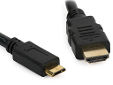
\includegraphics[width=3cm]{images/hdmi-cable.jpg}
    \captionof{subfigure}{HDMI}
  \end{minipage}%
  \hspace{0.03\textwidth}
  \begin{minipage}{0.2\textwidth}
    \centering
    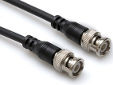
\includegraphics[width=3cm]{images/sdi-cable.jpg}
    \captionof{subfigure}{SDI}
  \end{minipage}%
  \hspace{0.03\textwidth}
  \begin{minipage}{0.2\textwidth}
    \centering
    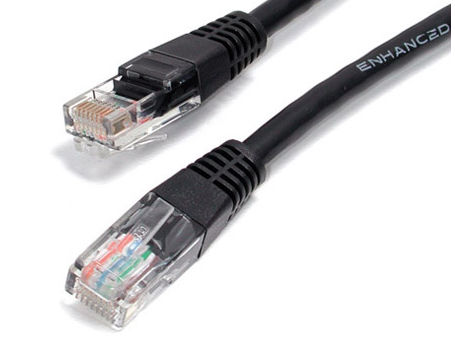
\includegraphics[width=3cm]{images/ethernet-cable.jpg}
    \captionof{subfigure}{Ethernet}
  \end{minipage}%
  \hspace{0.03\textwidth}
  \begin{minipage}{0.2\textwidth}
    \centering
    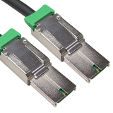
\includegraphics[width=3cm]{images/pcie-cable.jpg}
    \captionof{subfigure}{PCIe}
  \end{minipage}
  \caption{Illustration des différents connecteurs utilisées par Vahana VR}
\end{figure}


\section{Réalisation}
\subsection{Architecture de la solution}
Il s'agissait tout d'abord de saisir le concept de la Programmation Orientée Composant, et la manière
dont il est appliqué pour Vahana VR.\\
Cette approche propose d'utiliser différents \emph{composants}, ou \textit{plugins},
qui vont interragir entre eux~: ici les plugins entrées/sorties avec Vahana VR. On entend
par composant, des bibliothèques (fichiers .dll) qui peuvent être chargées et utilisées
par un programme client, ici Vahana VR. Tout comme les dépendances\footnote{Présentées dans 
la section \cf{integration-dependances-player}.}, un composant va fournir un ensemble
de fonctions, déclarées dans les \textit{headers} qui accompagnent les
fichiers bibliothèques compilés. Ces fonctions sont donc regroupées dans un module externe
au logiciel qui peut y faire appel si besoin, ou non.\\
L'intérêt d'une telle approche est qu'elle permet de développer les plugins séparément du logiciel
logiciel client. Un composant peut également être réutilisé par d'autres programmes~: en ce sens, la POC trouve
des similitudes avec la POO\footnote{Programmation Orientée Objet}.\\
Enfin, si l'analogie avec les dépendances pouvait être faite jusqu'ici, contrairement à ces
dernières dont l'utilisation est réalisée \enquote{en dur} dans le code, un composant
peut être remplacé ou d'autres ajoutés. En effet, le programme recense les composants
présents et tente de les charger \emph{dynamiquement} selon une interface attendue, celle du
\textit{header}~: le code de la bibliothèque est inconnu car compilé, seul sont
connue les fonctions attendues du composant.\\
Un exemple de plugins, est typiquement les extensions d'un navigateur web. Ces composants
ont été écrits pour le navigateur, en répondant à une interface attendue par ce logiciel,
et peuvent être activés ou désactivés à volonté par l'utilisateur.\\
\newline
Concrètement, un plugin pour Vahana VR est composé en trois parties~:
\begin{itemize}
  \item Une interface pour créer une entrée.
  \item Une interface pour créer une sortie.
  \item Une interface \textit{discovery} dont le rôle est d'indiquer les possibilités
    de créations entrées/sorties.
\end{itemize}
Ainsi, lors de son exécution, Vahana VR va chercher les bibliothèques présentes dans le dossier
\mintinline{shell-session}{plugins} à sa racine et charge celles présentant ces interfaces.\\

\subsection{Conception type d'un plugin}
sdk, driver, programme test

doc, samples

reader

writer

discovery

\subsection{Quelques difficultés et solutions spécifiques}
yuan et wrapper

decklink et design pattern decorator

loadunpacker teledyne

ximea cuda


\section{Déploiement}
\subsection{Création du dépôt VideoStitch-IO}
annexe A
comment fixé builds et update.sh

\subsection{Documentation}
grandes lignes, comment shippé avec plugin et vahana

\subsection{Tests et \textit{QA} de l'intégration des plugins}


\section{Bilan et suite}


\chapter{Conclusion}
\epigraph{Il semble que la perfection soit atteinte, non quand il n'y a plus 
rien à ajouter mais quand il n'y a plus rien à retrancher}{--- \small{\textup{Saint-Exupéry,
Terre des hommes}}}

\section{Conclusion technique}

\section{Conclusion personnelle}


\appendix

\bibliographystyle{unsrt}
\bibliography{bibliographie}

\addcontentsline{toc}{chapter}{Bibliographie}


\listoffigures
\addcontentsline{toc}{chapter}{Table des figures}

\end{document}

